\documentclass[
% -- opções da classe memoir --
12pt,				% tamanho da fonte
openright,			% capítulos começam em pág ímpar (insere página vazia caso preciso)
oneside,			% para impressão em recto e verso. Oposto a oneside
a4paper,			% tamanho do papel.
% -- opções da classe abntex2 --
% chapter=TITLE,		% títulos de capítulos convertidos em letras maiúsculas
% section=TITLE,		% títulos de seções convertidos em letras maiúsculas
% subsection=TITLE,	% títulos de subseções convertidos em letras maiúsculas
% subsubsection=TITLE,% títulos de subsubseções convertidos em letras maiúsculas
% -- opções do pacote babel --
english,			% idioma adicional para hifenização
french,				% idioma adicional para hifenização
spanish,			% idioma adicional para hifenização
brazil,				% o último idioma é o principal do documento
]{abntex2}


% ---
% PACOTES
% ---

% ---
% Pacotes fundamentais
% ---
\usepackage{lmodern}			% Usa a fonte Latin Modern
\usepackage[T1]{fontenc}		% Selecao de codigos de fonte.
\usepackage[utf8]{inputenc}		% Codificacao do documento (conversão automática dos acentos)
\usepackage{indentfirst}		% Indenta o primeiro parágrafo de cada seção.
\usepackage{color}				% Controle das cores
\usepackage{graphicx}			% Inclusão de gráficos
\usepackage{microtype} 			% para melhorias de
% justificação
\usepackage{amsmath}
\usepackage{xltxtra}
% \setmainfont{Source Han Sans CN}
% \usepackage{xeCJK}
% ---
% \usepackage[UTF8]{ctex}
% \usepackage{xeCJK}
% \setCJKmainfont{SimSun}
% ---
% Pacotes de citações
%\usepackage{graphicx}
\usepackage{grffile}
\usepackage{longtable}
\usepackage{wrapfig}
\usepackage{rotating}
\usepackage[normalem]{ulem}
\usepackage{amsmath}
\usepackage{textcomp}
\usepackage{amssymb}
\usepackage{capt-of}
\usepackage{hyperref}
\usepackage{xltxtra}
\setmainfont{Source Han Sans CN}
\usepackage[brazilian,hyperpageref]{backref}	 % Paginas com as citações na bibl
\usepackage[alf]{abntex2cite}	% Citações padrão ABNT
\usepackage{graphicx}
\usepackage{graphics}

% ---
% Pacotes adicionais, usados no anexo do modelo de folha de identificação
% ---
% \usepackage{multicol}
% \usepackage{multirow}
% ---

% ---
% Pacotes adicionais, usados apenas no âmbito do Modelo Canônico do abnteX2
% ---
% \usepackage{lipsum}				% para geração de dummy text
% ---


% ---
% CONFIGURAÇÕES DE PACOTES
% ---

% Enumeração extendível
\usepackage{enumitem}
\setlist{nolistsep}

% Caminho dos arquivos-imagem
\graphicspath{
  {./Imagens/}
  {./Imagens/Linux}
  {./Imagens/WM}
  {./Imagens/BenchMarks}
  {./Imagens/Running}
}

% ---
% Configurações do pacote backref
% Usado sem a opção hyperpageref de backref
\renewcommand{\backrefpagesname}{Citado na(s) página(s):~}
% Texto padrão antes do número das páginas
\renewcommand{\backref}{}
% Define os textos da citação
\renewcommand*{\backrefalt}[4]{
  \ifcase #1 %
  Nenhuma citação no texto.%
  \or
  Citado na página #2.%
  \else
  Citado #1 vezes nas páginas #2.%
  \fi}%
% ---

% ---
% Informações de dados para CAPA e FOLHA DE ROSTO
% ---
\titulo{Softwares Livres na Academia e na Indústria}
\autor{PEDRO GOMES BANQUINHO \\ Orientador: Dr. Wei-Liang Qian}
\local{Lorena,}
\data{2021}%13 de Fevereiro de 2020}
\instituicao{%
  Universidade de São Paulo - USP \\
  Escola de Engenharia de Lorena
  \par
  Tese de Conclusão de Curso}
\tipotrabalho{Monografia}
% O preambulo deve conter o tipo do trabalho, o objetivo,
% o nome da instituição e a área de concentração
% \preambulo{Relato da elaboração e progresso do minicurso de \LaTeX}
% ---

% ---
% Configurações de aparência do PDF final

% alterando o aspecto da cor azul
\definecolor{blue}{RGB}{41,5,195}

% informações do PDF
\makeatletter
\hypersetup{
  % pagebackref=true,
  pdftitle={\@title},
  pdfauthor={\@author},
  pdfsubject={\imprimirpreambulo},
  pdfcreator={Pedro G. Branquinho},
  pdfkeywords={tese}{software}{livre},
  colorlinks=true,       		% false: boxed links; true: colored links
  linkcolor=blue,          	% color of internal links
  citecolor=blue,        		% color of links to bibliography
  filecolor=magenta,      		% color of file links
  urlcolor=blue,
  bookmarksdepth=4
}
\makeatother
% ---

% ---
% Espaçamentos entre linhas e parágrafos
% ---

% % O tamanho do parágrafo é dado por:
\setlength{\parindent}{0.8cm}

% % Controle do espaçamento entre um parágrafo e outro:
\setlength{\parskip}{0.2cm}  % tente também \onelineskip

% ---
% compila o indice
% ---
\makeindex
% ---

% ----
% Início do documento
% ----
\begin{document}

% Seleciona o idioma do documento (conforme pacotes do babel)
% \selectlanguage{english}
\selectlanguage{brazil}

% Retira espaço extra obsoleto entre as frases.
\frenchspacing

% ----------------------------------------------------------
% ELEMENTOS PRÉ-TEXTUAIS
% ----------------------------------------------------------
% \pretextual

% ---
% Capa
% ---
\imprimircapa
% ---

% ---
% RESUMO
% ---

% resumo na língua vernácula (obrigatório)
\setlength{\absparsep}{18pt} % ajusta o espaçamento dos parágrafos do resumo
\begin{resumo}

  Demonstrou-se como é possível construir uma série de aplicações
  baseada em softwares de licença livre, à partir de um sistema
  aberto, o Linux com inteface EXWM - Emacs X Window Manager. Além
  disso, foi propiciado casos reais de aplicações na Indústria e no
  investimento privado, autônomo. Bem como, utilizações na Academia,
  à nível de lecionar, e pequisa. Sustenta-se que a economia aberta
  possui similaridade estrutural ao movimento \textit{Open Source} e
  seu desenvolvimento, o que aponta que essa é e continuará a ser,
  paulatinamente mais, o paradigma de desenvolvimento econômico
  tecnológico. Assim, imprescindível à formação do engenheiro.
  
  \noindent
  \textbf{Palavras-chaves}: software livre. automação. freqtrade. idústria. academia.

\end{resumo}
% ---


% ---
% inserir lista de ilustrações
% ---
\pdfbookmark[0]{\listfigurename}{lof}
\listoffigures*
\cleardoublepage
% ---

% ---
% inserir o sumario
% ---
\pdfbookmark[0]{\contentsname}{toc}
\tableofcontents*
% ---


% ----------------------------------------------------------
% ELEMENTOS TEXTUAIS
% ----------------------------------------------------------
\textual

% ----------------------------------------------------------
% Introdução (exemplo de capítulo sem numeração, mas presente no Sumário)
% ----------------------------------------------------------
\chapter[Introdução]{Introdução}
% \addcontentsline{toc}{chapter}{Introdução}

Na formação de um engenheiro físico, o qual, por definição, é um profissional generalista, os softwares abertos (FOSS - Free and Open Source Software) e a participação da comunidade Open Source são detrimentais para sua formação.

A diversidade os quais softwares extensíveis acarretam (\autoref{sec:diversidade}) podem mudar completamente a experiência do usuário, e o trazer mais próximo do papel de desenvolvedor. Essa experiência não necessita de ser exclusiva de cientistas da computação ou profissionais de TI. Pois, a programação pode ser encarada tanto como ciência e arte \cite{knuth1968art}.

Os Softwares Abertos possuem quatro liberdades pétreas \autoref{sec:opensource}, garantindo os direitos de estudo, cópia, modificação e redistribuição.

Bem como a ciência se beneficia com seus rápidos avanços, de uma comunidade global de participantes, com as mais distintas especializações profissionais. Também, beneficia-se a computação com a comunidade aberta, e especialização eclética, tanto de membros quanto de softwares.

% <<O que são os softwares livres e como se aplicam no contexto acadêmico e industrial>>

% É notório o fato de que optimizações 


\section{Objetivo}

% Demonstrar a importância dessa categoria de softwares, e da comuniadade aberta, no desenvolvimento tecnológico.
Demonstramos a defassagem que um profissional de engenharia apresentaria, sem forte formação dentro da computação. Ademais, ao partir da gama de aplicações, em estado da arte, as quais são partilhadas de forma aberta e livre, pretende-se reinterar o caso da necessidade de compreensão do fenômeno dos softwares abertos. Pois, essa lógica e dinâmica não possui paralelos nem na economia, nem na comunidade científica \cite{hippel2003open,peters2009open}.

Há até debates acirrados sobre o sentido de \textit{Open Science}, um termo que recentemente se popularizou e o qual constitui claro paralelo com o movimento \textit{Open Source}. Porém, mal compreendido e, raramente, debatido sob esse prisma, dentro das ciências sociais. Cita-se o mais citado dos artigos na busca no Google Scholar ``The future(s) of open science'', o qual somente cita três vezes o termo Open Source, em tom dismissivo \cite{mirowski2018future}. Assim, argumenta-se que a formação básica do engenheiro na área da computação precisa ser sólida, bem como o entendimento das forças que moldaram esse movimento, de forma a poder entender o futuro em que caminhamos, de forma crítica.




\section{As interconexões das aplicações e o OS}

\subsection{Por quê o GNU/Linux nos importa?}
Discutiremos introdutoriamente na monografia, o que é o sistema operacional
GNU/Linux, e o por quê de ser a porta de entrada à comunidade Open
Source. Primeiramente, o GNU/Linux é o primeiro e maior sucesso da lógica
de negócio Open Source \cite{tu2000evolution,west2001open} - dessa forma,
utilizá-lo é uma maneira de entender como a lógica de negócio
dependente de comunidades abertas funcionam \cite{fink2003business}.

Além do mais, o novo usuário-desenvolvedor de GNU/Linux,
inerentemente, tem de aprender sobre outros softwares os quais vêm
conjunto à sua distribuição - o que aumenta sua adoção
\cite{west2001open}. Desta forma, sente-se compelido a participar e
estender os comportamentos do programa \cite{hertel2003motivation}.

Para aquém da sua inicial expressão filosófica de liberdade, o
GNU/Linux hoje é o \textit{standard} em empresas te alta
tecnologia. E, sua lógica de negócio, por mais que desafie os moldes
empresariais econômicos do \textit{status quo}, sem sombra de dúvidas
funciona, traz resultados às empresas, a economia e à
comunidade. Usar-se do GNU/Linux, então, é uma maneira de se inserir
nesse novo contexto lógico econômico
\cite{moody2009rebel,hippel2003open,peters2009open}.

\subsection{Como as aplicações de alto nível se beneficiam de um \textit{OS}}

Na hierarquia de softwares e aplicações, os sistemas operacionais
podem ser vistos como um meta-aplicação.

``The evaluator, which determines the meaning of expressions in a
programming language, is just another program.'' \cite{abelson1996structure}

Existem níveis, ou camadas, de abstração em virtualmente qualquer
aplicação. Ou seja, o conceito de meta-programação e torres de
interpretadores é um problema um tanto quanto comum, e possui
implicações diretas no uso dos softwares.

Os sistemas operacionais, como o GNU/Linux, uma camada essencial
nessa torre de interpretadores. Em especial, eles se comunicam com
\textit{firmwares} - softwares de baixa expressividade e alta performance, os
quais controlam \textit{hardwares}. Também, comunicam-se com softwares de alta
expressividade, os quais comprazem as aplicações escritas, ou
estendidas, pelo usuário-desenvolvedor do sistema. Por conseguinte, o
Sistema Operacional possui um papel de mediador entre softwares de
alto e baixo nível - como são chamados pela literatura - o que
configura-os como uma espécie de \textit{middleware}.

\begin{figure}[ht]
  \centering
  \caption{\label{fig:tower} Esquemática de uma torre de interpretadores}
  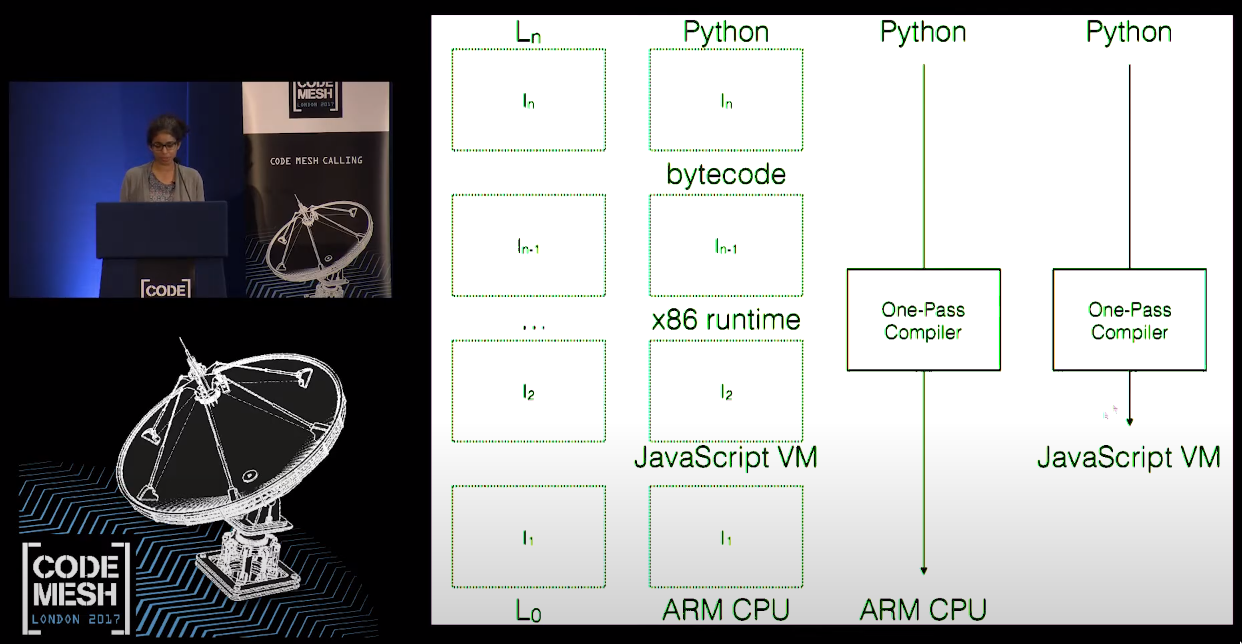
\includegraphics[width=\linewidth]{torres.png}
  \legend{Code Mesh, apresentação Towers of Interpreters, por Nada Amin}
\end{figure}

O problema característico de concatenar sistemas de softwares um sob o
outro introduz complexidades em termos de manter compatibilidade entre
versões de programas e sua performance. O estudo desses comportamentos
e suas soluções teóricas possuem um ramo próprio, desvinculado, por
exemplo, de quais linguagens compõe a torre, ou qual aplicação estamos
lidando \cite{amin2017towers}. O que se interessa é com o
comportamento final do sistema, e se é possível colapsar o sistema.

\begin{figure}[ht]
  \centering
  \caption{\label{fig:tower2} Categorização do estudo de torres de interpretadores}
  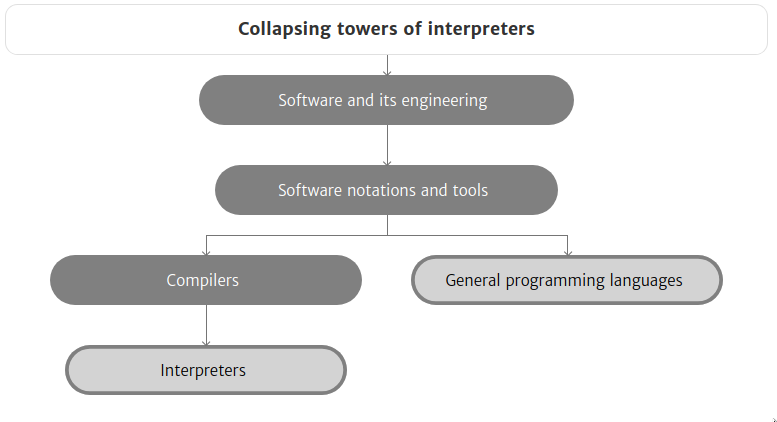
\includegraphics[width=0.5\linewidth]{torres2.png}
  \legend{Fonte: \cite{amin2017towers}}
\end{figure}


Finalmente, os O.S. consistem em grandes colapsadores de torres de
interpretação. Encontram-se encarregados de colapsar firmware,
middlewares e softwares de alto nível. Por fim, o quão bem um sistema
operacional conduz essa tarefa, tanto mais a experiência do usuário
final é facilitada.

\begin{figure}[ht]
  \centering
  \caption{\label{fig:os} Torre de interpretadores e os Sistemas Operacionais.}
  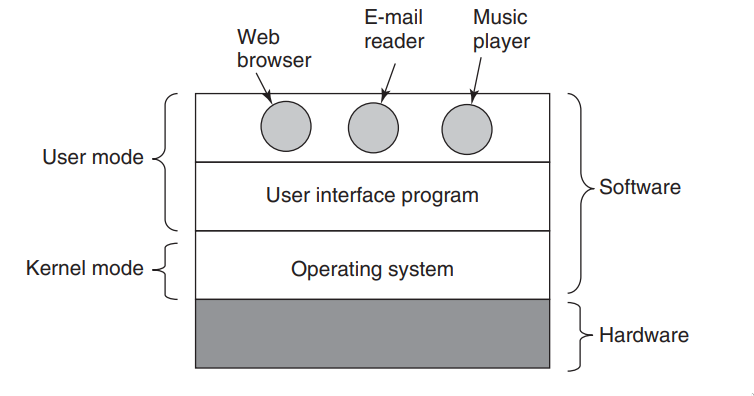
\includegraphics[width=0.5\linewidth]{tower-os.png}
  \legend{Fonte: \cite{tanenbaum2015modern}}
\end{figure}

\begin{citacao}
If every application programmer had to understand how all these things work in detail, no code would ever
get written. Furthermore, managing all these components and using them optimally
is an exceedingly challenging job. For this reason, computers are equipped with a
layer of software called the operating system, whose job is to provide
user programs with a better, simpler, cleaner, model of the computer
and to handle managing all the resources just mentioned. \cite{tanenbaum2015modern}
\end{citacao}


\section{Da influência da educação na adoção}

É claro, na literatura, de que a adoção dos softwares open source no
setor industrial
dependem da competência, e do quão profundo seus conhecimentos
precisam ser para resolução de seus problemas
\cite{li2013all,gallego2015open,spinellis2012organizational}. 

Ao mesmo tempo, a adoção depende diretamente das inclinações
intrínsecas da equipe de TI \cite{racero2021can}.

Por fim, por mais que cursos profissionalizantes no tópico aumente a
intensidade e rapidez de sua adesão, por alunos
\cite{racero2020predicting} e profissionais inclinados à autonomia
\cite{gallego2015open}, a adoção final está mais ligada a fatores
intrínsecos de motivação. No entanto, é importante notar a existência de um
efeito-rede em adoções \cite{spinellis2012organizational} e.g., quanto mais semelhantes adotam
OSS, maior a chance de adoção.




\section{Performance e futuro do open source como motivos de adoção}

Delineia-se que existe um ganho em performance ao se utilizar a
plataforma GNU/Linux em comparação ao Windows \cite{sulaiman2021comparison}. Porém, mais importante
ainda, é o fato de que os principais benefícios não estão no sistema
operacional em si, mas no treino que se obtém quando se utiliza um
sistema totalmente dependente de ferramentas e comunidades
abertas.

Pois, é nesse momento que se dá a transformação profissional
indivíduo, ao mesmo tempo que se aumenta a chance das empresas que
esse profissional irá trabalhar de adotarem OSS. Mesmo que, as
empresas em geral, e as de software em particular, beneficiam-se
grandemente da comunidade aberta e livre ao mesmo tempo que não
precisam e não incentivam nenhum direto incentivo ao trabalho da
comunidade \cite{hauge2008adoption}.

\section{O perfil do engenheiro e dos usuários de FOSS}

É notável que dado a profundidade que se procura a dar a formação,
ainda em nível de graduação, do engenheiro físico, espera-se que ele
seja um ideal candidato ao uso de FOSS. Pois, necessita de ambos de
inclínio a autonomia \cite{schrape2019open,racero2020predicting}, quanto profundidade em seu trabalho técnico,
para fomentar a necessidade e adoção de FOSS, em nível individual
\cite{li2013all,gallego2015open}.

\section{Como podemos alavancar o potencial de OSS na Indústria e Academia}

No presente trabalho, utilizou-se de diversas demonstrações de
conceitos, onde o autor desenvolveu e estendeu aplicações
desenvolvidas num contexto livre e aberto. Também, discute-se como se
integrar e acrescentar à comunidade aberta. Nota-se o quão fundamental
e significante são as conexões profissionais que se faz nesse nicho.

\chapter{Revisão Bibliográfica}
\section{Open Source}
\label{sec:opensource}
Qualquer programa que permita o usuário-programador ter as seguintes
liberdades:

\begin{enumerate}
\item Direito de rodar o programa, como você desejar, para qualquer fim.
\item Direito ao acesso ao código-fonte, para estudá-lo.
\item Direito de cópia e distribuição.
\item Direito à modificação do software.
\end{enumerate}

De maneira prática, a comunidade Open Source, fundamentalmente, se baseia no compartilhamento de suas configurações. As vantagens de existirem inúmeras outras pessoas utilizando o mesmo software é de que a melhoria da fronteira do programa é expandida de forma acrescida, em comparação a de um time restrito de usuários.

\subsection{Diversidade}
\label{sec:diversidade}

Dado que um direito fundamental dos softwares livres é a modificação e propagação das versões modificadas, existe uma diversidade de expressividade, sem paralelos em outras áreas da tecnologia.

Por exemplo, uma parte de software fundamental na configuração de um computador é seu gerenciador de interfaces (Window Manager). Onde, um programa é devotado a gerenciar como outros programas gráficos devem se dispor na tela de computador.

Enquanto sistemas operacionais (Operational Systems) privados, como Windows e MacOS possuem versões lançadas frequentemente - vinte e cinco versões lançadas de Windows. O Windows possui apenas quatro versões, com suporte ativo \cite{wikipedia_2021W}.

São vinte lançamentos de MacOS, e quatro verões mantidas \cite{wikipedia_2021Mac}.

Essa estreiteza de versões se dá, dentre os fatores, pois os usuários são cerciados do direito de extender ou alterar os comportamentos programados no sistema. Assim, vítimas do suporte descontinuado e de sua atualização de versões restritivas.

Em contra partida, existem, paralelamente, por volta de 278 distribuições de Linux \cite{wikipedia_2021Linux}. Onde, existem as distribuições raízes, com princípios e filosofias de desenvolvimentos teóricos e práticos diferentes.

Assim, bem como em qualquer outro escopo de software, a variação dos softwares abertos e livres (FOSS) sempre serão superiores aos monopolizados.


\section{O Linux}

Existem distribuições raízes de linux, das quais muitas distribuições existem como ramificações. Nomeia-se, de forma genêrica, devido aos princípios base de uma classe de distribuições, como famílias. Cita-se algumas das mais influentes e populares, Red Hat Linux, Debian, CentOS, Fedora,Pacman-based, OpenSUSE, Gentoo-based, Ubuntu-based, Slackware, Open Sourced-based e as distribuições Independetes.

É possível apreciarmos visualmente a riqueza de distribuições pela \autoref{fig:linux-genealogy}.

\begin{figure}[!htb]
  \caption{\label{fig:linux-genealogy} Genealogia Distribuições Linux}
  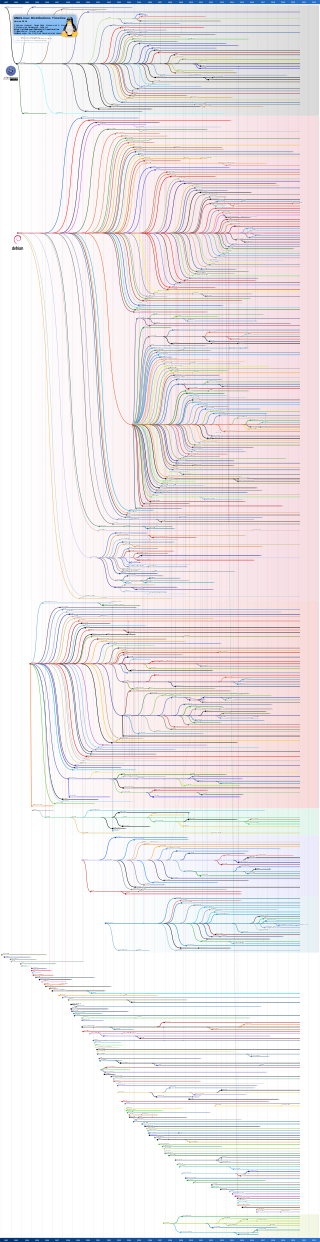
\includegraphics[height=\textwidth, angle=-90]{diversidade}
  \legend{Histórico de evolução das distribuições Linux \cite{wikipedia_2021Linux}}
\end{figure}

\subsection{\label{sec:origem-linux} Origem Histórica}
O projeto do GNU/Linux iniciou-se separadamente, por duas frentes. O
GNU - abreviação de, GNU's Not Unix - por usuários revoltados com o
sistema de seguraça dos computadores do MIT (Laboratory of Computer
Science - LCS) \cite{stallman2002my,emacswiki2021history}. Dentre
eles, o ainda ativo Richard Stallman, após já dez anos de evolução do
editor de texto \cite{emacswiki2021history}.

Paralelamente, Linus Torvalds desenvolveu um sistema operacional
portável aberto, como sua tese de mestrado
\cite{torvalds1997linux}. Por fim, houve uma junção dos projetos, os
quais colaboravam o Linux, como sistema operacional, e GNU com todas
as aplicações utilitarias do sistema \cite{stallman1997}.


\subsection{O Emacs}

Como foi visto na \href{sec:origem-linux}, o projeto GNU possuia muitas utilidades as quais foram incorporadas ao kernel Linux, para dar corpo a um sistema operacional. O Emacs, particularmente, caracteriza um dos primeiros softwares extensivamente estendidos dentro do projeto. Sendo classificado como um editor de texto, escrito em Elisp, o qual é um dialeto da família de linguagens Lisp.

Por mais que seja um editor de texto, por natureza, dada a larga possibilidade de expansão de suas utilidades, existem pacotes e maneiras de o configurar como um sistema completo de Window Manager. Ou seja, pode-se servir como interface gráfica e gerenciadora de outras aplicações.

\begin{figure}[ht]
  \centering
  \caption{\label{fig:exwm1} EXWM - Emacs X Window Manager}
  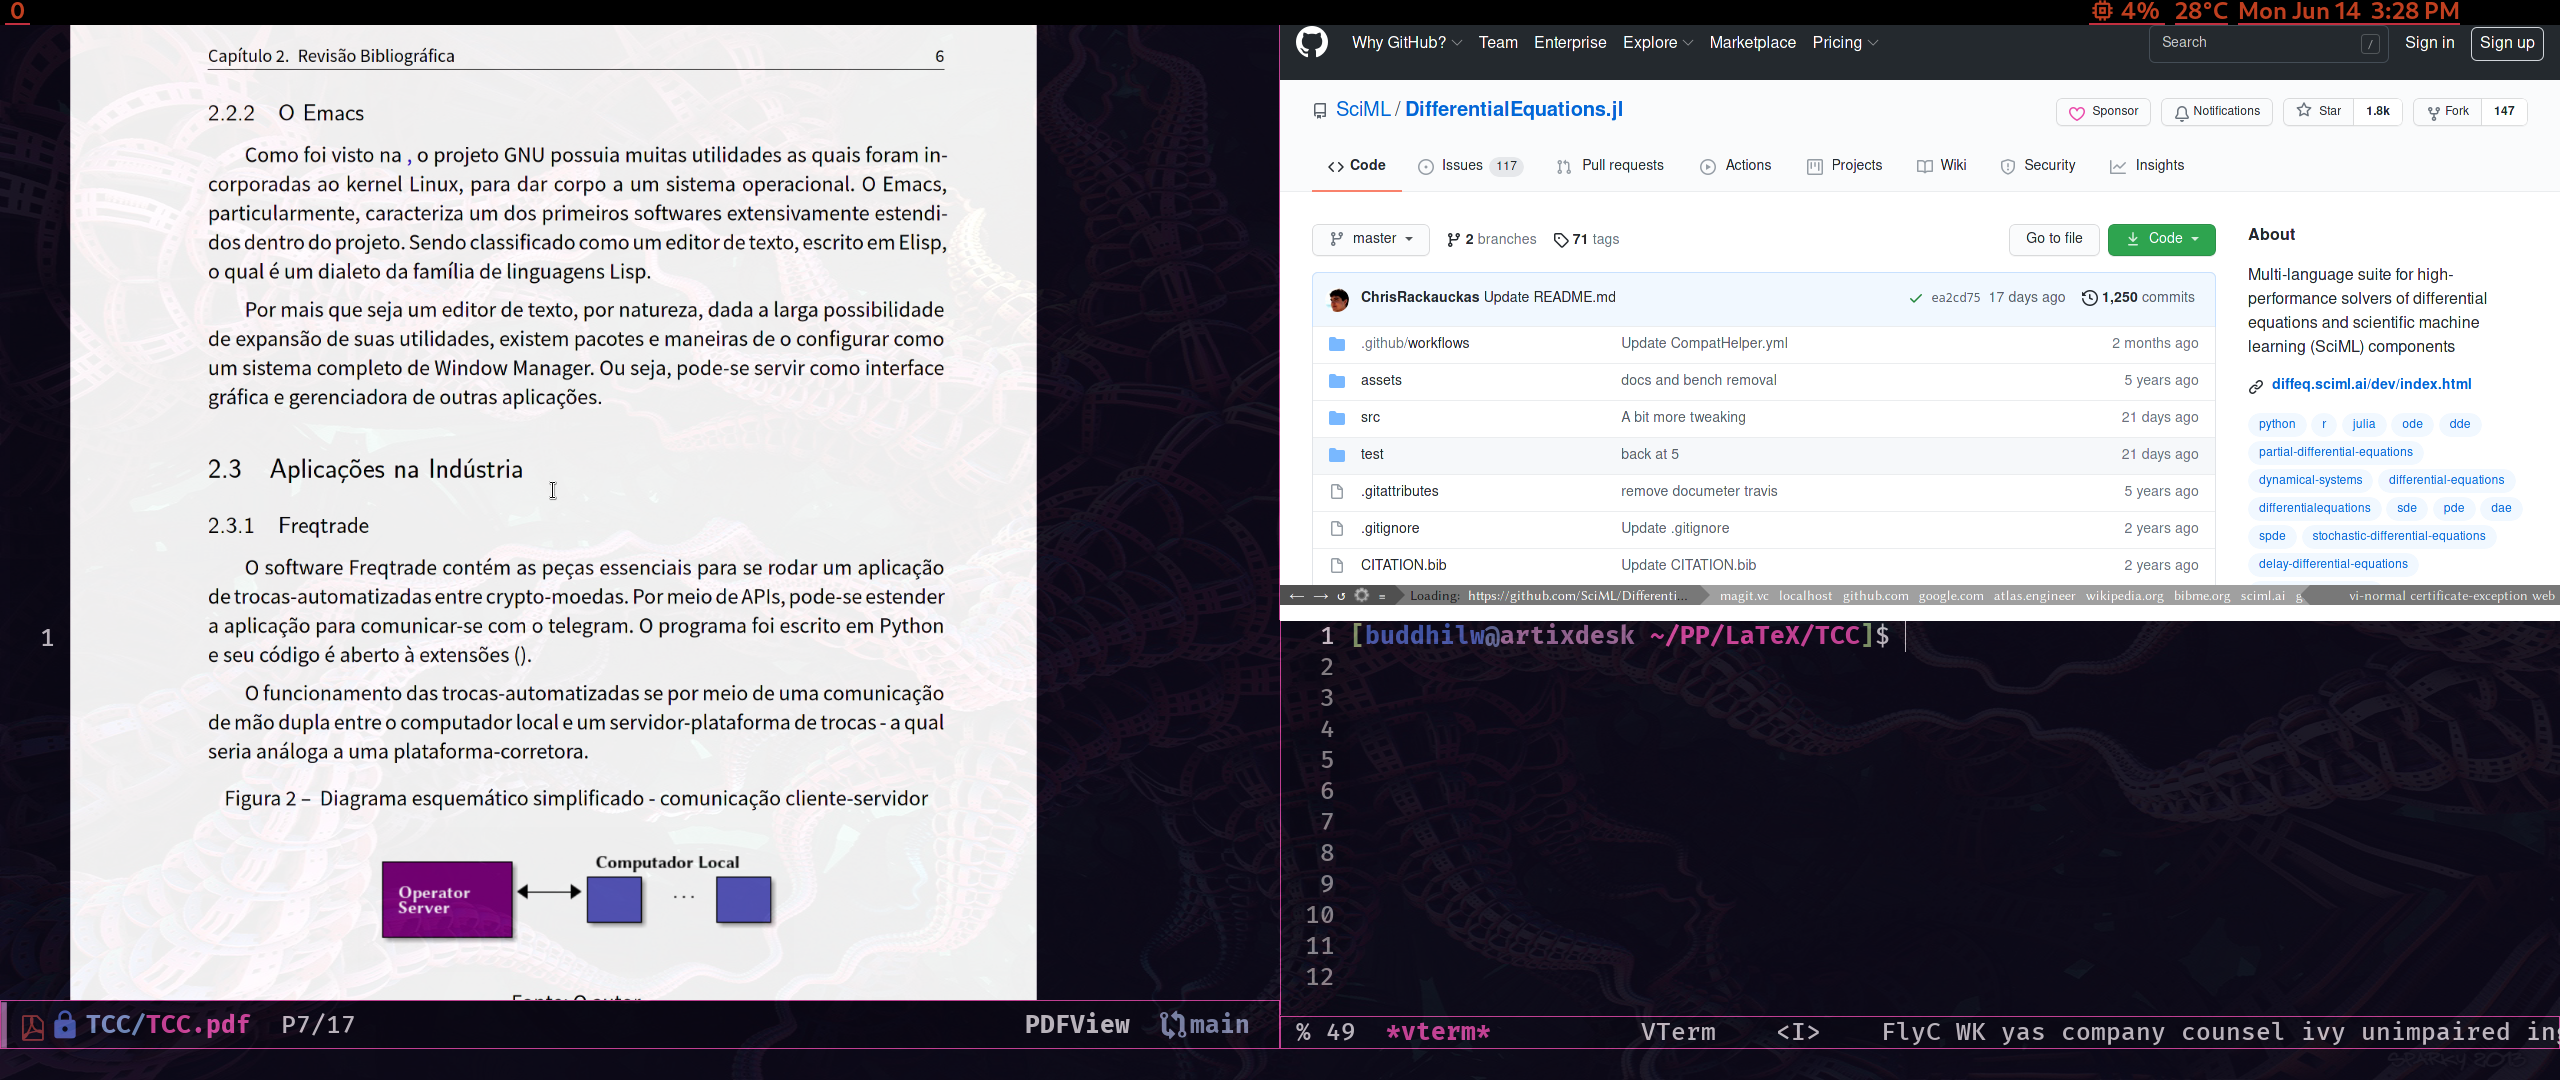
\includegraphics[width=\linewidth]{exwm2.png}
  \legend{Fonte: foto do ambiente de WM do autor.}
\end{figure}

A \autoref{fig:exwm1} é um exemplo do ambiente de desktop totalmente manuseado por meio do Emacs, utilizando-se do EXWM. Pode-se notas que é possível rodar browsers modernos, bem como renderizadores de imagens e PDF.

\section{Comparações entre a performance e adoção de sistemas
  operacionais}

\subsection{Performance}
Quando testado em termos de eficiência, o Windows 10 performa-se bem
abaixo do Linux, em tarefas em nível de usuário \cite{sulaiman2021comparison}.

Em um mesmo hardware, os programas que são
executados no pano de fundo, continuamente, pelo Windows consumem um
valor próximo de 5\%  de CPU e 41\% de RAM. Enquanto, no Linux Mint - uma
versão popular de Linux - o consumo é de 1.8\% de CPU e 24\% de
RAM. Uma diferença de performance de mais de mais de 200\% em CPU e
aproximatamente 200\% em RAM \cite{sulaiman2021comparison}.

A execução de um programa escrito em VBS - relacionado aos programas
do pacote Office -, se dá com uma diferença de 0.501 segundos para o Linux
Mint e 4.75 segundos no Windows. E.g., existe uma diferença absoluta de
$\frac{4.75-0.501}{0.501}=423\%$ em performance \cite{sulaiman2021comparison}.

Por fim, também existem pesquisas feitas com rigor técnico em todas as
outras área de manuseação de \textit{firmwares/harwares}, como
\textit{wireless} \cite{SDevan2013WINDOWS8V}; paralelismo e
manuseação de aplicações em servidores \cite{aveleda2010performance};
programas científicos (Fast Fourier Transform) et al
\cite{d2011performance}; performance em arquiteturas de Realidade Virtuais (VR)
\cite{thubaasini2010efficient} etc. Todas elas demonstram uma
performance superior na renderização e/ou no tempo de renderização em
plataformas GNU/Linux
\cite{aveleda2010performance,thubaasini2010efficient,SDevan2013WINDOWS8V,sulaiman2021comparison,d2011performance}.

\subsection{Demografia da adoção de FOSS}

Fritzgerald enunciou em 2006 que o perfil de adoção dos sistemas open
source estava numa fase ``OSS 2.0'', o qual transcendera a
generalização de que isso era algo inutilizável pela pessoa média e
uma ferramenta exclusiva de ``\textit{hackers}''
\cite{fitzgerald2006transformation}. E, que ainda haveriam
conseguintes transformações até um patamar \textit{mainstream}. Isto
é, se tornaria um lugar comum na sociedade e industria, e que grande
parte do desenvolvimento seria de autoria de grandes empresas.

Em 2008, foi feita uma pesquisa sobre a adoção da indústria de
softwares, na Finlândia. Em contraste à caracterização de
Fritzgerald, 50\% das empresas utilizavam amplamente de Open Source
Software, porém, a participação era quase nula na comunidade
aberta. Por fim, mais de 30\% dessas empresas participantes relatavam que 40\%
do ganho era fruto de produtos e serviços desenvolvidos pela
comunidade aberta\cite{hauge2008adoption}. É importante se notar que
eram empresas de pequeno e médio porte, em sua maioria.

Em 2012, um estudo em grande empresas - mil companias listadas na revista US
Fortune - derivou algumas conclusões \cite{spinellis2012organizational}:

\begin{itemize}
\item A adoção está diretamente associada à equipes de TI com
  trabalhos os quais demandam expertise e conhecimentos extensivos
  especializados, bem como busca por eficiência \cite{gallego2015open,
 li2013all}.
\item Aumento exponencial, à partir de um ponto de acumulação;
\item Existe um efeito-rede responsável pela adoção nas grandes.
empresas;  
\end{itemize}

Assim, a adoção em empresas de pequeno, médio e grande porte variam
grandemente, e não possuem efeitos notáveis na expansão do
movimento. No entanto, ainda são positivamente influenciadas por ele
\cite{spinellis2012organizational,hauge2008adoption,fitzgerald2006transformation}. A
maior influência positiva no movimento, indica-se, é dado por pequenas
empresas \cite{kshetri2004economics}. 

Observa-se no entando, de 2012 ao presente, uma intensificação de
adoção e ubiquidade da adoção dessas tecnologias abertas \cite{schmidt2016agile}. São
consideradas, atualmente, o berço inovatório da indústria de softwares
\cite{schrape2019open,schmidt2016agile}.

Pesquisas mais recentes determinam que, independente do tamanho da
empresa, a adoção da empresa depende diretamente do treinamento dos
agentes de TI e sua inclinação por autonomia
\cite{racero2020predicting}. Finalmente, a adoção e crença na
efetividade desses softwares depende de fatores principalmente
intrínsecos e independem de treinamento, por mais que os treinamentos
em OSS potencializa a adoção de usuários inclinados ao uso
\cite{racero2021can}.

\section{Demonstração de Aplicações na Indústria}
\subsection{Freqtrade}
O software \emph{Freqtrade} contém as peças essenciais para se rodar
um aplicação de trocas-automatizadas entre crypto-moedas. Por meio de
APIs, pode-se estender a aplicação para comunicar-se com o
telegram. O programa foi escrito em Python e seu código é aberto à
estensão, possuindo centro e quarenta e sete contruibuidores, com existência datando de Maio de 2017 \cite{fang2020cryptocurrency}.

O funcionamento das trocas-automatizadas se por meio de uma
comunicação de mão dupla entre o computador local e um
servidor-plataforma de trocas - a qual seria análoga a uma
plataforma-corretora.

\begin{figure}[ht]
  \centering
  \caption{\label{fig:diagrama-freqtrade} Diagrama esquemático simplificado -
    comunicação cliente-servidor}
  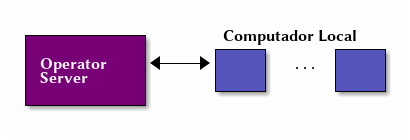
\includegraphics[width=0.6\linewidth]{Imagens/server-client-fq_4.png}
  \legend{Fonte: O autor.}
\end{figure}

Grande parte do trabalho de se escrever um robô autômato, para
qualquer fim, compraz em programar protocólogos de comunicação com
servidores. Pois, o robô deverá ser capaz de dizer o servidor quais
operações devem ocorrer, tanto gerando respostas ao cliente - dados a
serem armazenados no computador local -, quanto operações internas ao
servidor - como, executar uma compra e venda de criptomoeda.

\begin{figure}[ht]
  \centering
  \caption{\label{fig:diagrama-freqtrade2} Diagrama esquemático -
    comunicação cliente-servidor}
  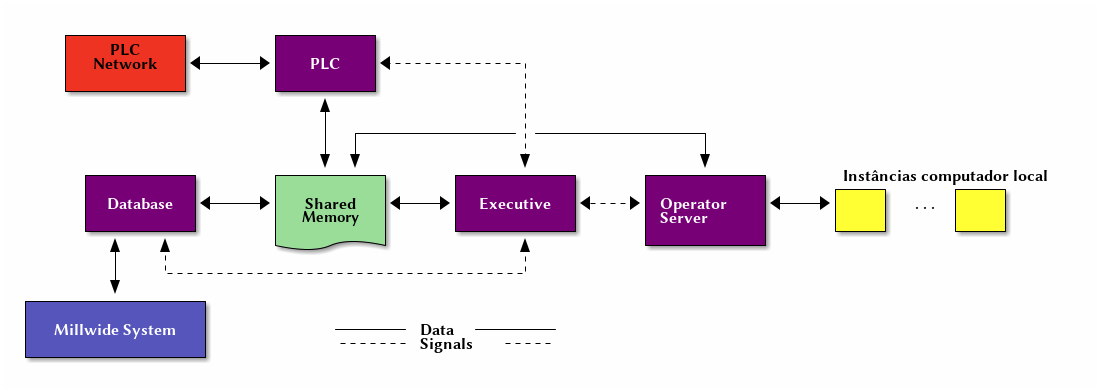
\includegraphics[width=1\linewidth]{ditaa_4.png}
  \legend{Fonte: O autor.}
\end{figure}

Assim, um diagrama completo o qual captura essa complexidade poderia
esquematicamente ser visto na \autoref{fig:diagrama-freqtrade2}.

Ao se utilizar o software aberto, toda essa complexidade da
\autoref{fig:diagrama-freqtrade2} se torna mais próxima à
\autoref{fig:diagrama-freqtrade}, pois toda a abstração-estrutural já
se encontra escrita. Basta, para quem decidir utilizar o programa ler,
entender e modificar o conteúdo disponível na documentação do projeto.


% <<No que consiste o software; os métodos utilizados para seu funcionamento>>

\subsection{OR-Tools}
\label{sec:ortools}

A ferramenta OR-Tools traduz-se em bibliotecas largamente desenvolvida
pela comunidade aberta, e a empresa Google \cite{}; utilizável em C++,
Python, Java, (Clojure), C\#, .Net.

OR-Tools possui a utilidade de resolver problemas como agendamento de
horários, o qual, estruturalmente, assemelha-se aos algorítimos de
solução de problemas como Sudoku \cite{}.

De forma geral, esses problemas caem dentro de um ramo da matemática e
computação chamado Problemas de Optimazação Constrita
(\textit{Constraint Optimization})

\section{Demonstração de Aplicações Acadêmicas}

% \clearpage
\subsection{DifferentialEquations.jl}

A biblioteca numérica DifferentialEquations possui uma das melhores performances de softwares numéricos que existem \cite{rackauckas2017differentialequations}. Sua performace é comparativa à implementações em FORTRAN e C. Existem \textit{ports} da biblioteca para Python e R, porém, desenvolveu-se em Julia.

Dentre a categoria de problemas possíveis de se resolver, utilizando-se ferramentas próprias do pacote, lista-se  as seguintes categorias de equações diferenciais \cite{rackauckas2019confederated,rackauckas2017adaptive,rackauckas_stability-optimized_2018,sykora2020stochasticdelaydiffeq,rackauckas2018comparison,rackauckas2019diffeqflux,rackauckas2020universal,gowda2019sparsity,ma2021modelingtoolkit},

\begin{itemize}
\item Equações discretas (Estocásticos discretos (Gillepie/Markov), e mapas funcionais)
\item Equações diferenciais ordinárias (ODEs)
\item Equações estocásticas ordinárias (Integrações simpléticas, Método IMEX)
\item Equações estocásticas diferenciais algébrigcas (SODEs or SDEs)
\item Equações diferenciais aleatórias (RODEs ou RDE)
\item Equações diferenciais algébricas (DAEs)
\item Equações diferenciais com retardo (DDEs)
\item Equações diferenciais neutras, retardadas e algebricamente retardadas (NDDES, RDDEs e DDAEs)
\item Equações diferenciais estocásticas retardadas (SDDEs)
\item Suporte parcial de soluções em equações diferenciais estocásticas neutras, retardads e retardadas algebraicas (SNDDEs, SRDDEs, SDDAEs)
\item Equações mistas discretas e contínuas (\textit{Jump Diffusions})
\item Equações diferenciais parciais (estocásticas) ((S)PDEs) - ambas com portabilidade de métodos finitos e/ou diferenças finitas)
\end{itemize}


% Discrete equations (function maps, discrete stochastic (Gillespie/Markov) simulations)
% Ordinary differential equations (ODEs)
% Split and Partitioned ODEs (Symplectic integrators, IMEX Methods)
% Stochastic ordinary differential equations (SODEs or SDEs)
% Stochastic differential-algebraic equations (SDAEs)
% Random differential equations (RODEs or RDEs)
% Differential algebraic equations (DAEs)
% Delay differential equations (DDEs)
% Neutral, retarded, and algebraic delay differential equations (NDDEs, RDDEs, and DDAEs)
% Stochastic delay differential equations (SDDEs)
% Experimental support for stochastic neutral, retarded, and algebraic delay differential equations (SNDDEs, SRDDEs, and SDDAEs)
% Mixed discrete and continuous equations (Hybrid Equations, Jump Diffusions)
% (Stochastic) partial differential equations ((S)PDEs) (with both finite difference and finite element methods)

\subsubsection{Portabilidade em Julia}

Para se utilizar do pacote, basta utilizar os seguintes comandos

\begin{verbatim}
# Carrega o gerenciador de pacotes, Pkg e instala, se preciso, o pacote.
using Pkg
Pkg.add("DifferentialEquations")
# Porta as utilidades do pacote, sem necessitar de referí-lo no meio do código
using DifferentialEquations
\end{verbatim}

\subsubsection{Portabilidade em Python}

Num terminal, utilizando-se do gerenciador de pacotes pip,
\begin{verbatim}
pip install diffeqpy
\end{verbatim}

Num terminal, rodando-se o interpretador de Python,
\begin{verbatim}
>>> import diffeqpy
>>> diffeqpy.install()
\end{verbatim}

Por fim, opcionalmente, utilize numba para aumentar a performance do código,
\begin{verbatim}
pip install numba
\end{verbatim}

Ademais, apenas repita o comando, dentro de um aquivo python,

\begin{verbatim}
import diffeqpy
\end{verbatim}

\subsubsection{Portabilidade em R}

Para instalação,
\begin{verbatim}
install.packages("diffeqr")
\end{verbatim}

Na primeira chamada de,
\begin{verbatim}
diffeqr::diffeq_setup()
\end{verbatim}

Será feito o download do DifferentialEquations.jl. Um subconjunto específico do pacote é ativamente mantido \href{https://cran.r-project.org/web/packages/diffeqr/index.html}{no CRAN}.

\subsection{O \LaTeX}

O \LaTeX{} possui separação entra as tarefas de produção de um
documento. A linguagem permite-nos separar as tarefas de formatação do texto, da escrita de seu conteúdo. Desta forma, o usuário concentra-se
exclusivamente em seu conteúdo, em um estágio da escrita do documento. E, na formatação de sua aparência, em outro momento.

Assim, ganha-se em qualidade de produção. Bem como, ganha total autonomia sob o documento, pois a programação da disposição gráfica dos elementos textuais pode ser programada - isto é, modificada indefinidamente, a partir dos comportamentos padrões dos pacotes utilizados. O sistema tipográfico de \LaTeX{} chegou a ser considerado o sistema digital de
tipografia mais sofisticado que existe, devido a essa paradigma de
programação funcional, \textit{bottom-up} \cite{haralambous2007}.

O \LaTeX, tecnicamente, é a junção do sistema de tipografia \TeX,
inventado por Donald Knuth, para tipografia de alto nível
\cite{knuth1986}; com os poderosos macros que facilitam a extensão do programa \TeX, a qual damos o nome de
\LaTeX. O \LaTeX{} foi inicialmente desenvolvido por Leslie Lamport, com
seus pacotes fundamentais de formatação \cite{lamport1994}. O \LaTeX,
por conseguinte, não é somente uma linguagem de tipografia de alto
nível, mas também um conjunto de macros para facilitar a tipografia em
si. Qualifica-se, assim, como um sistema de preparação de documentos;
uma linguagem markup de domínio específico.

\subsubsection{Classe Canônica ABNT de produção científica}

Documentos sob os requisitos das normas ABNT (Associação Brasileira de Normas
Técnicas) para elaboração de documentos técnicos e científicos
brasileiros - como artigos científicos, relatórios técnicos, trabalhos
acadêmicos, como teses, dissertações, projetos de pesquisa e outros
documentos do gênero \cite{abntex2012} - é ao que se chama classe
canônica ABNT.

\begin{citacao}
  Os documentos indicados tratam-se de “Modelos Canônicos”, ou seja,
  de modelos que não são específicos a nenhuma universidade ou instituição, mas
  que implementam exclusivamente os requisitos das normas da ABNT, Associação
  Brasileira de Normas Técnicas. \cite[Cap. 1]{araujoclasse}
\end{citacao}

% \clearpage

As normas as quais prescrevem o modelo canônico são:

\begin{itemize}
\item \textbf{ABNT NBR 6022:2018:} Informação e documentação -
  Artigo em publicação periódica científica - Apresentação.
\item \textbf{ABNT NBR 6023:2002:} Informação e documentação -
  Referência - Elaboração.
\item \textbf{ABNT NBR 6024:2012:} Informação e documentação -
  Numeração progressiva das secções de um documento - Apresentação.
\item \textbf{ABNT NBR 6027:2012:} Informação e documentação -
  Sumário - Apresentação.
\item \textbf{ABNT NBR 6028:2003:} Informação e documentação -
  Resumo - Apresentação.
\item \textbf{ABNT NBR 6029:2006:} Informação e documentação -
  Livros e folhetos - Apresentação.
\item \textbf{ABNT NBR 6034:2004:} Informação e documentação -
  Índice - Apresentação.
\item \textbf{ABNT NBR 10520:2002:} Informação e documentação -
  Citações.
\item \textbf{ABNT NBR 10719:2015:} Informação e documentação -
  Relatórios técnicos e/ou científico - Apresentação.
\item \textbf{ABNT NBR 14724:2011:} Informação e documentação -
  Trabalhos acadêmicos - Apresentação.
\item \textbf{ABNT NBR 15287:2011:} Informação e documentação -
  Projeto de pesquisa - Apresentação.
\end{itemize}

% \begin{figure}[t]
%   \caption{\label{im:6} Imagens escritas com Tikz, representação de um
%     arbusto}
%   \begin{center}
%     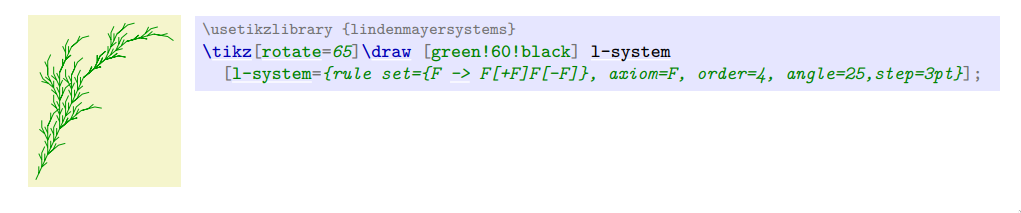
\includegraphics[width=\linewidth]{./Imagens/5.png}
%   \end{center}
%   \legend{Fonte:
%     \href{http://linorg.usp.br/CTAN/graphics/pgf/base/doc/pgfmanual.pdf}{Manual
%       Tikz, CTAN}}
% \end{figure}


\section{Trabalhos Canônicos na Área de Computação}
\subsection{Structure and Interpretation of Classical Mechanics (SCIM)}
\label{sec:scim}
A bilioteca científica de simulações de mecânica clássica, em Scheme (um dialeto de Lisp), foi escrito com intento de ser utilizado em cursos de mestrado no MIT. Acompanhado à biblioteca, existe o livro, o qual serve de material didáctico ao curso \cite{sussman2015structure}.

\subsection{Structure and interpretation of computer programs (SICP)}
O curso de Scheme (SICP), o qual é ensinado como materia básica de computação no MIT, possui como acompanhantes um dos mais influentes livros já escritos na história da computação \cite{abelson1996structure}. O curso é pioneiro em aprofundar-se epistemologia da programação. Onde, o uso de Scheme, o qual possui notação uniforme para todas as funcionalidades da língua foi revolucionário. Conquanto, em contraste aos outros cursos de fundamentos da computação focavam em ensinar a linguagem mais amplamente utilizada no momento.

O curso SCIM (\autoref{sec:scim}) foi um precursor de SICP. O curso continua ativo e o livro continua a ser utilizado amplamente no MIT, e em inúmeras outras faculdades. Uma lista não exaustiva pode ser encontrada em \url{https://mitpress.mit.edu/sites/default/files/sicp/adopt-list.html}, em que pelo menos, vinte universidades o adotam, em mais de oito países.

\subsection{SICMUtils - Portabilidade de (SCIM) em Clojure}
Existe uma biblioteca reescrita em clojure, a qual porta as funcionalidades descritas na biblioteca científica SCIM \cite{sicmutils2016github}. Essa biblioteca é escrita numa das mais modernas linguages de computação com adoção amplamente da Industria, Clojure. Recentemente, a maior empresa utilizado de Clojure até então, a Cognitect, a qual inventou a língua foi comparada pelo Nubank \cite{clojure2020}.

A língua é tão poderosa que as implementações não são apenas numéricas, nem são somente simbólicas. É possível utilizar-se da mesma função (\textit{procedure}) para se fazerem cálculos numéricos ou simbólicos, tendo apenas de se mudar os argumentos de entrada (\textit{inputs}).

\clearpage



\chapter{Materiais e Métodos}
O planejamento da monografia seguiu as seguintes etapas:

\begin{enumerate}
\item Contato e estratégias com o orientador;
\item Determinação do tópico principal; 
\item Delineação específica dos subtópicos;
\item Organização da agenda à partir das datas finais objetivadas;
\item Início à escrita do TCC;
\item Junção de notas exploratórias sobre o tópico;
\item Pesquisa bibliografia;
\item Escrita de todos os tópicos da monografia;
\item Revisão contínua à cada etapa da monografia;
\item Organização de apresentação;
\end{enumerate}

\section{Convite ao orientador}
Procurou-se um docente tanto familiar ao autor, quanto versado e
interessado no tópico de pesquisa.

\section{Delineação do tema}
Dado que o tema softwares livres na indústria e academia é um tópico
indefinidamente abrangente, houve uma necessidade imprescindível de
delimitar graduamente o tópico.

Nas revisões contínuas, determinava-se o quão profundo tinha se
abordado os tópicos, e se era necessário dar procedência, ou seguir o
andamento de outras parte da agenda.

\section{Organização cronológica}
Decidiu-se por seguir o método de diagrama de Gantt, amplamente
utilizado em organização de projetos. As partições temporais foram
ponderadas pelas datas limites objetivadas.

\section{As fases da escrita da Monografia}
Como a monografia se caracteriza como uma Análise Exploratória, o
enfoque foi na literatura concernente ao Tema.

Na subtópico acadêmico, procurou-se dar enfoque ambos softwares auxiliares
de pesquisas, quanto úteis à sala de aula. Bem como, pretendia-se
explicar conceitos-chave na compreensão da dinâmica histórica e atual
do ecossistema em que se desenvolve e aplicam softwares.

Ademais, nas aplicações tecnológicas, o autor documentou softwares que
já utilizou em situações reais.

\section{Junção de notas}
Ao se utilizar os softwares os autores havia produzido anotações sobre
o desenvolvimento do software. Uma auto-documentação, enquanto se
desenvolvia, ou se estudava os mecanismos de uma aplicação. Assim,
utilizou-se dessas notas para construção da monografia.

\section{Pesquisa bibliográfica}
A revisão da bibliografia objetiva facilitar o entendimento da
indústria dos softwares, a qual é difere em seu aspecto
majoritariamente livre e aberto. Além do mais, procurou-se fazer um
recorte de história, usos e desenvolvimento em estado da arte de
diversos softwares icônicos.

A maior quantidade de informações históricas encontra-se armazenada
digitalmente, em sites de instituições internacionais, como o
GNU. Conquanto, nas aplicações procurou-se o embasamento em artigos
científicos.

Utilizou-se do Google Scholar e a plataforma da ACM (Association for
Computing Machinery), da qual o autor é
membro e na qual existe material especializado em computação e softwares.

\section{Revisão contínua}
Parte fundamental da organização da monografia foi a troca de
informações, auxílio, e integração constante das considerações do
orientador Dr. Wei-Liang.
\section{Organização da apresentação}
Na apresentação, procura-se utilizar ferramentas interativas e
demonstração de conceitos por meio de programação em tempo real
aplicações. Escolheu-se utilizar da ferramento Org-mode, integral ao
Emacs.

\chapter{Resultado e Discussões}

\section{Convite ao orientador}
O autor já havia interagido com o Dr. Wei-Liang, o qual no passado
havia pedido, a titulo de pesquisarem juntos, que se instalasse o
sistema operacional do Linux. Ademais, uma das aplicações era na
resolução e simulação de sistemas resolvidos por Lagrangeanas - tópico
lecionado pelo orientador, na disciplina de Mecânica Clássica.

Assim, fortunamente o orientador se sentiu inclinado a participar
desse trabalho. E, concorda que o ensino sobre a iniciativa Open
Source, bem como os softwares em si, são detrimentais na vida acadêmica.

\section{Delineação do tema}

A iniciativa GNU e o open source é indefinidamente abrangente. Existem
softwares abertos escritos para virtualmente qualquer outra área do
exercício cognitivo do ser humano.

Necessitou contentar-se em parcialmente mostrar aplicações mais em
mão, as quais seriam mais relevantes ao escopo da monografia. Bem
como, optou-se por aprofundar-se em tópicos já utilizados na vida do
autor para se resolver problemas na academia e na indústria.

Assim, a delimitação principal se deu entorno de ferramentas abertas
das quais, na indústria foram apresentados OR-Tools e
Freqtrade.

\subsection{Da Indústria}
As línguas utilizadas para o desenvolvimento desses softwares foram
Python e C++. Porém, no caso de OR-Tools existe portabilidade para
C++ (nativo), Python, Java, .NET. Todos os projetos e línguas possuem licença aberta.

OR-Tools destina-se a resolver um problema virtualmente
conspícuo a qualquer negócio ou estrutura social prestadora de
serviço. Pois, o problema de agendamento de horários, com condições de
restrições impostas, é extremamente comum. Por exemplo, para organizar
turnos de funcionários, em uma empresa; turnos de enfermeiros em um
hospital - exemplo dado na própria documentação do software etc.

Freq-trade destina-se a automação de investimentos em
crypto-moedas. A ferramenta surgiu espontaneamente da comunidade
aberta, sem incentivo algum externo - até, pois, não existe um
responsável que chefia o projeto. E, num curto período de
desenvolvimento, cinco anos, desde 2017, a aplicação conta com
inúmeras otimizações computacionais, e APIs com interfaces como
Telegram. Não existe paralelo de software fechado o qual é
comercializado, com mesmo escopo.

\subsection{Da academia}
\label{subsec:res-academia}

Optou-se a estudar aplicações escritas em Python, Julia,
Clojure(script). Pois, o autor possui histórico de
utilização dessas ferramentas. Com efeito, a pesquisa constituiu, em
grande parte, na junção de todos os esparços projetos em que o autor
já havia colaborado ou desenvolvido. E, no aprofundamento da
compreensão de todas esses projetos, para que fosse possível fazer uma
apresentação coesa do ferramental utilizado.

Os programas em Julia possuiam cunho numérico. Pois, sua computação
optimizada compara-se a performance de FORTRAN e C++. Assim, o
principal pacote estudado foi DifferentialEquations.jl, a qual pode
ser utilizada para resolver uma gama de equações diferenciais,
incluindo a categoria Estocástica.

O programa em Python é de processamento de imagens. Escolheu-se essa
aplicação, pois demonstra o quão abrangente é a portibilidade de
programas escritos em outras línguas ao Python - principalmente,
devido a grande comunidade de cientistas e programadores que o
utilizam.

\subsection{A intersecção}

Com Clojure(Script), Bash e \LaTeX{}, foi possível criar tanto
simulações que estendem a compreensão de fenômenos físicos do campo
abstrato ao visual. Também, empregou-se de Closh e Babashka, duas
bibliotecas de Clojure dedicadas a interoperabilidade com Bash, a qual
se processava milhares de arquivos, por meio de pipelines de
arquitetura complexas. Assim, facilitando a escrita de uma quantidade
enorme de relatórios técnicos na área de segurança do trabalho. 

Quanto a Clojure(Script), foram pesquisadas simulações gráficas, as
quais inerentemente são simples de se programar em Clojure. Pois, seu
ecossistema pode interoperar entre JVM (Java Virtual Machine) e
JavaScript. Assim, dado que ambos Java e JavaScript foram as línguas
mais populares por décadas, existem uma enorme quantidade de ambientes
e bibliotecas a nossa disposição. Bem como, Clojure é uma Lisp - e,
caracteristicamente, essa família é utilizada para prototipagem, vide
AutoCAD escrito em AutoLisp.

Dado que existem bibliotecas dedicadas a Mecânica Clássica em nível de
mestrado, bem como exite capacidades de se renderizar conceitos
físicos abstratos. Então, decorreu-se a computação de programas que
demonstravam conceitos de Física, Cálculo, e Computação Generativa.


\section{Organização cronológica}

A organização do projeto se deu utilizando os diagramas de Gantt, e as
agendas dinâmicas, /org-agenda/, nativas do Emacs. Por conseguinte,
toda a comunicação sobre o projeto foi materializado por meio de
cronogramas e agendas.

\section{As fases da escrita da Monografia}
Iniciou-se a escrita da monografia pela pesquisa bibliográfica, dado
que a pesquisa se categoriza, epistemologicamente, como uma Análise
Exploratória. O \textit{template} utilizado para escrita do projeto
foi o \abnTeX{}, biblioteca do \LaTeX dedicado a escrita de documentos sob as normas ABNT.

\section{Junção de notas}
O \textbf{org-mode} é uma ferramenta de organização e anotação, desenvolvida
para pesquisa e reprodutibilidade de pesquisas. Assim, todas as etapas
de desenvolvimento do projeto foram desenvolvidas e documentas utilizando
essa ferramenta.

A documentação implícita ao desenvolvimento é uma
característica fundamental e pensada do Org-mode. Pois, segue o
paradigma de \textit{Literate Programming}. Assim, há uma mistura de
notas e códigos em um mesmo ambiente. Fazendo que a prototipação do
código seja automaticamente documentável.

Por fim, é possível exportar qualquer anotação de extensão .org para
.tex e consequentemente .pdf. Assim, reutilizar dessas anotações foi
uma tarefa natural.

\subsection{Aplicações em Clojure}

\subsection{Aplicações em Julia}
\subsection{Aplicações em Python}

\section{Pesquisa bibliográfica}
A pesquisa bibliográfica foi em grande parte encontrada em sites sem
autores. Pois, a documentação foi criada ou pela comunidade, ou por
instituições, não unicamente publicada em formato de livro ou artigo.

Da parte acadêmica, como o pacote de resolução de equações
diferenciais, em Júlia, encontrou-se vasta literatura. Até porque, a
língua foi criada para resolver problemas computacionais tocantes
principalmente a comunidade científica do MIT.

Por fim, algumas ferramentas apenas existem documentadas e contidas
inteiramente em repositórios, como o Github. Foram os casos do
OR-Tools e as simulações em Clojure. São publicações puramente eletrônicas.

\section{Revisão contínua}

Dentro do cronograma concebido para desenvolvimento da monografia,
pôs-se metas e etapas de escrita do documento. E, estipulou-se os
conteúdos necessários para cada nova versão do documento, aliado a uma
data limite. Assim, o retorno do orientador ao orientado pode se dar
mais frequentemente.

\section{Organização da apresentação}

Como se está utilizando de diversas ferramentas e extensões dentro do
Emacs e do Org-mode, em particular, optou-se por utilizar uma de suas
funcionalidades dedicada a apresentações. 

\chapter{Conclusão}
Dentro das iniciativas Open Sourced, existem virtualmente aplicações
para todas as áreas das aventuras do ser humano. Isto é, seja o uso de
computação gráfica, processamento de imagens, expressões artísticas,
ou ferramentas de organização, há um software escrito para esse fim.

É observável a falta de competição quanto a quantidade e qualidade de
softwares fechados e abertos. Ademais, a capacidade de
extensão dos softwares livres, por meio das quatro fundamentais
liberdades de suas licenças, permitem que exista uma variedade imensa
de uso de uma mesma ferramenta. Por fim, o enriquecimento dessa
participação colaborativa solidifica e generaliza as ferramentas
abertas - num grau e rapidez inimagináveis, comparados ao processo de
desenvolvimento por uma equipe fechada.

Demonstrou-se diversos usos desses software, sem paralelos, na
Indústria e na Academia. Ambos possuem algorítimos na fronteira da
ciência, a qual o uso apenas é limitado pela imaginação e capacidade
formativa do usuário-desenvolvedor. Assim, é imprescindível que no
curso de engenharia se tenha uma ampla formação com base nos softwares
livres, sob os quais a computação moderna subiste.

Apontou-se algumas portas de entrada, fundamentais, a esse paradigma,
os sistemas com Kernel Linux, as aplicações GNU as quais lhe dão
roupagem, e por fim os sistemas sociais onde se desenvolve os
softwares, como a plataforma de versionamento Git/Github. Ademais,
demonstrou-se, com efetividade, que é possível construir e rodas todas
essas aplicações num sistema totalmente aberto.

\bibliography{bib}


\end{document}

%%% Local Variables:
%%% mode: latex
%%% TeX-master: t
%%% End:
